\documentclass{beamer}
\usetheme{LANL}

%/../imc/draco/environment/latex/

\AtBeginSection[]
{
  %\setcounter{tocdepth}{1}
  \begin{frame}<beamer>
    \frametitle{Outline}
    \tableofcontents[currentsection,currentsubsection,hideothersubsections]
  \end{frame}
  %\setcounter{tocdepth}{2}
}

\title[Implementing a Discrete Maximum Principle]{Implementing a\\ Discrete
Maximum Principle\\ for the IMC Equations}
\author{Paul W. Talbot \\
\texttt{talbotp@engr.orst.edu\\ \\
Allan Wollaber \\
\texttt{wollaber@lanl.gov}}}
\date{\today}
\subtitle{A Summer Internship}
\institute{Under the mentorship of \\ Dr. Allan Wollaber\\
  \texttt{wollaber@lanl.gov} \\\ \\Los Alamos National Laboratory}
\reportnum{}

\begin{document}

\begin{frame}
 \titlepage
\end{frame}

\begin{frame}\frametitle{Outline}\tableofcontents[pausesections]
\end{frame}


\section{The Need for the DMP}
\begin{frame}\frametitle{Why a Maximum Principle?}
\begin{columns}
\begin{column}{0.5\textwidth}
\begin{figure}
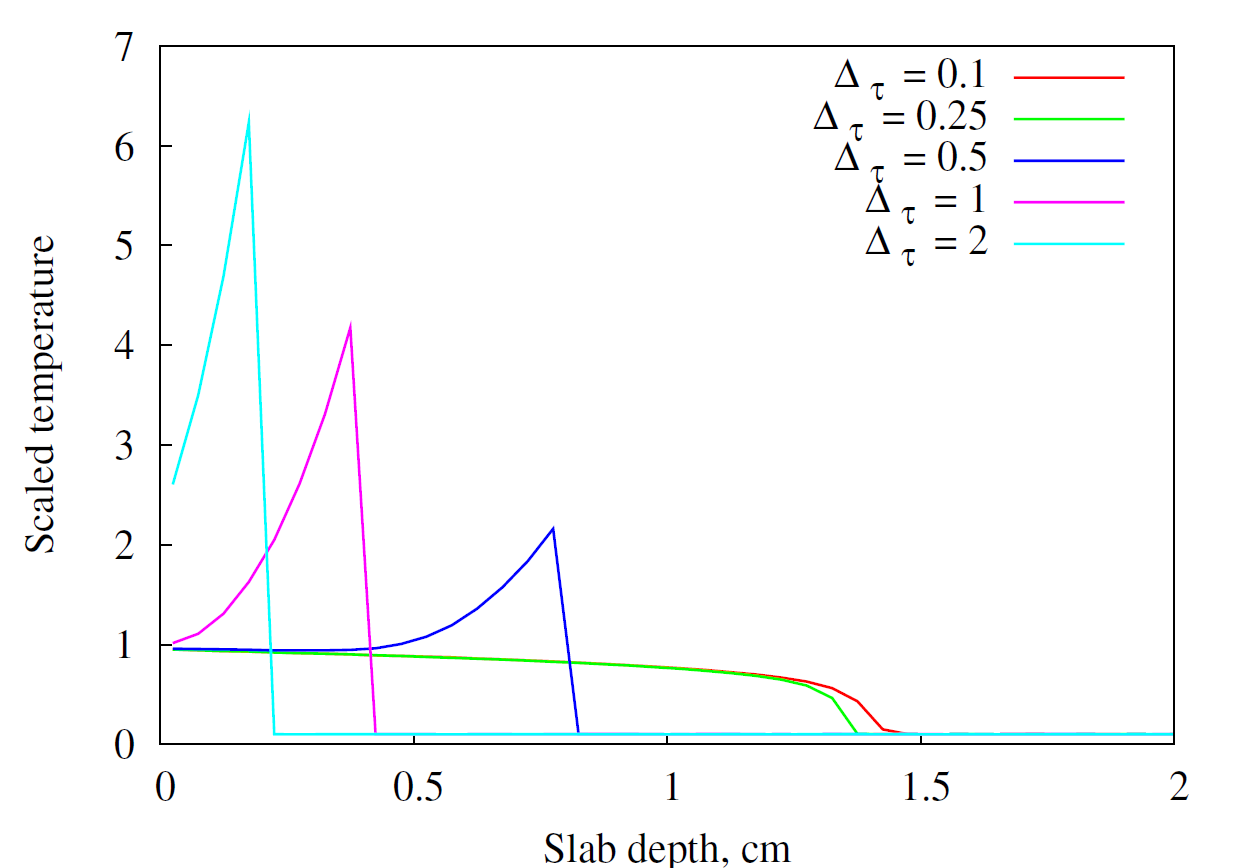
\includegraphics[width=\linewidth]{DMP_viol_dt}
\end{figure}
\end{column}
\begin{column}{0.5\textwidth}
\begin{figure}
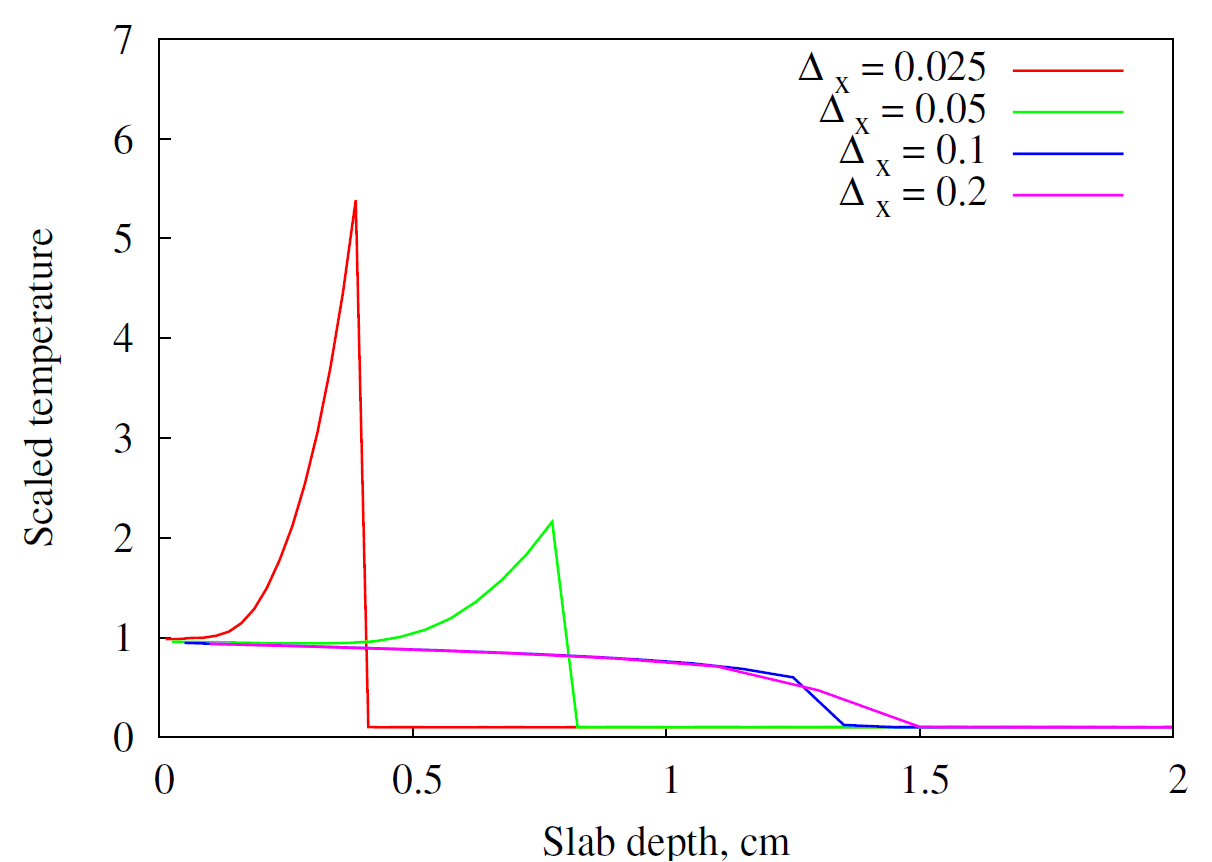
\includegraphics[width=\linewidth]{DMP_viol_dx}
\end{figure}
\end{column}
\end{columns}
\end{frame}



\section{Previous Maximum Principles}
\begin{frame}\frametitle{History at a Glance}
  \begin{itemize}
    \item Fleck and Cummings\; \emph{(1971)}
    \item Larsen and Mercier\; \emph{(1987)}
    \item Wollaber, Larsen, and Densmore\; \emph{(2011)}
  \end{itemize}
\end{frame}
\subsection{Fleck and Cummings}

\begin{frame}\frametitle{History at a Glance}
  \begin{itemize}
    \item Fleck and Cummings\; \emph{(1971)}
  \end{itemize}
\pause
\begin{block}{Quote:}
\emph{The $ct=6$ cm curve is inaccurate near the source ... although the
remainder of the curve does not look bad.}
\end{block}
\end{frame}

\subsection{Larsen and Mercier}
\begin{frame}\frametitle{History at a Glance}
  \begin{itemize}
    \item Larsen and Mercier\; \emph{(1987)}
  \end{itemize}
\pause
\begin{exampleblock}{Continuous Maximum Principle}
\begin{equation*}
\Delta_t\leq \left[ \rho(T_n)-\alpha\beta_n\sigma_{p,n}\right]^{-1}
\end{equation*}
\end{exampleblock}

\begin{block}{Definitions}
\[\rho\equiv\int\int\sigma\frac{\mbox{max}(\Delta_B)}{\mbox{max}(\Delta_U)}\
    d\nu\ d\Omega\]
\begin{center}
\begin{tabular}{r l}
$\beta_n = \frac{4\phi_n}{c_v T_n}$ & %\hspace{40pt}
    $\sigma_{p,n}=\frac{4\pi\int\sigma_nB_n\ d\nu}{\phi_n}$ \medskip\\
$\phi_n=\int_{4\pi}I_nd\Omega$ &
    $\alpha=\mbox{``Implicitness'' Constant}$\medskip\\
$B=\mbox{Planckian Spectrum}$ & $U=\mbox{Material Energy Density}$
\end{tabular}
\end{center}
\end{block}
\end{frame}


\subsection{Wollaber, Larsen, and Densmore}
\begin{frame}\frametitle{History at a Glance}
  \begin{itemize}
   \item Wollaber, Larsen, and Densmore\; \emph{(2011)}
  \end{itemize}
\pause
\begin{exampleblock}{Discrete Maximum Principle}
\begin{equation*}
\Delta_t\leq\frac{c_v(T_u-T_0)}{R(\Delta_x,\Delta_t)-f_0c\sigma_paT_0^4}
\end{equation*}
\end{exampleblock}
\begin{block}{Definitions}
$R=$ Estimated Energy Deposited in Cell in $\Delta_t$ \\
$T_u=$ Incident Hot Radiation Temperature \\
$T_0=$ Initial Cell Material Temperature
\end{block}
\end{frame}

\begin{frame}\frametitle{History at a Glance}
\begin{block}{Comparison}
\begin{figure}
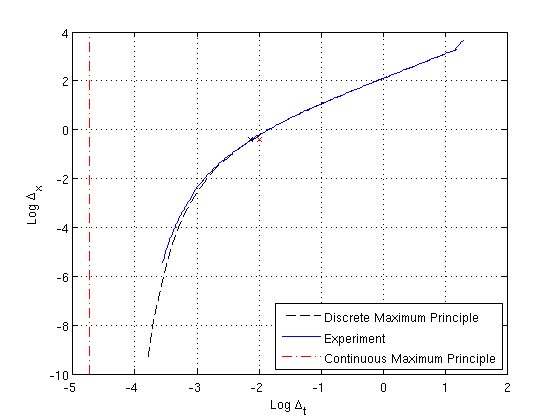
\includegraphics[width=0.57\linewidth]{CMP_DMP}
\caption{Continuous and Discrete Maximum Principles}
\end{figure}
\end{block}
\end{frame}


\section{Additions to the DMP}
\subsection{Term Truncation}
\begin{frame}\frametitle{Term Truncation}
\begin{exampleblock}{Energy Deposition}
$R(\Delta_x,\Delta_t)\equiv$
\[\frac{f_0\Delta_t2\pi}{\Delta_x}
  \int_0^\infty\frac{\sigma_0B_u}{\hat\Sigma}\left(\frac{1}{2}-
    E_3(\hat\Sigma\Delta_x)\right)d\nu \] \\
  \[+\frac{f_0\Delta_t\sigma_p}{\lambda^2\Delta_x}
    \left(-A\Delta_x-L\frac{1}{\hat\Sigma}\left(\frac{1}{2}
    -E_3(\hat\Sigma\Delta_x)\right)\right) \] \\
  \[+\frac{c_1f_0\Delta_t\sigma_p}{\lambda\Delta_x}
    (1-e^{-\lambda\Delta_x}) \] \\ \tiny
  \[+\frac{f_0\Delta_t\sigma_pL}{\Delta_x\lambda^4}\hat\Sigma
    \bigg(e^{-\lambda\Delta_x}\mbox{Ei}[(\lambda-\hat\Sigma)\Delta_x] +
    e^{\lambda\Delta_x}\mbox{Ei}[-(\lambda+\hat\Sigma)\Delta_x]
    -2\mbox{Ei}(-\Sigma \Delta_x)+
    \ln\frac{\hat\Sigma^2}{(\lambda+\hat\Sigma)|\lambda-\hat\Sigma|} \bigg).\]
\end{exampleblock}
\end{frame}
\begin{frame}\frametitle{Term Truncation}
\begin{exampleblock}{Energy Deposition, Revised}
\[R(\Delta_x,\Delta_t)\approx
\frac{f_0\Delta_t}{\Delta_x}\left(
  \zeta - \frac{\sigma_p}{\lambda^2} A\Delta_x
  + \frac{\sigma_p}{\lambda^2}\frac{1-f_0}{D}\zeta\right) \] \\
\end{exampleblock}
\begin{block}{Definitions}
\[\mbox{Equilibrium Constant } A\equiv-\lambda^2f_0\sigma_pacT_0^4\]
\[\mbox{Uncollided Flux Integral } \zeta\equiv\int_0^\infty \frac{\sigma_0
B_u}{\hat\Sigma}
  \left( \frac{1}{2}-E_3(\hat\Sigma\Delta_x)\right)\ d\nu \]
\end{block}
\end{frame}

\subsection{Initial Conditions}
\begin{frame}\frametitle{Generalized Initial Conditions}
\begin{block}{Before}
\[I(0,\mu,\nu,t)=2\pi B(\nu,T_u),\hspace{20pt}0<\mu\leq1,\; 0\leq t\]
\[I(\infty,\mu,\nu,t)=2\pi B(\nu,T_0),\hspace{20pt}-1<\mu\leq0,\; 0\leq t\]
\[I(x,\mu,\nu,0)=\alert{2\pi B_0}, \hspace{20pt}0\leq x\leq\infty,\; |\mu|<1\]
\end{block}\pause\transsplitverticalout
\begin{block}{Now}
\[I(0,\mu,\nu,t)=2\pi B(\nu,T_u),\hspace{20pt}0<\mu\leq1,\; 0\leq t\]
\[I(\infty,\mu,\nu,t)=2\pi B(\nu,T_0),\hspace{20pt}-1<\mu\leq0,\; 0\leq t\]
\[I(x,\mu,\nu,0)=\alert{2\pi B_R}, \hspace{20pt}0\leq x\leq\infty,\; |\mu|<1\]
\end{block}
\end{frame}

\begin{frame}\frametitle{Generalized Initial Conditions}
Changes:
\begin{block}{Before}
\[A\equiv-\lambda^2f_0\sigma_pacT_0^4\]
\end{block}
\begin{block}{Now}
\[\tilde A\equiv-\frac{acT_R^4}{c\Delta_tD}-\frac{f_0\sigma_pacT_0^4}{D}\]
\[\tilde R(\Delta_x,\Delta_t)=
\frac{f_0\Delta_t}{\Delta_x}\left(
  \zeta - \frac{\sigma_p}{\lambda^2} \tilde A\Delta_x
  + \frac{\sigma_p}{\lambda^2}\frac{1-f_0}{D}\zeta\right)\]
\end{block}
\end{frame}
\subsection{Multiple Gradients}
\begin{frame}\frametitle{Multiple Gradients}
\begin{itemize}
 \item Discrete Maximum Principle follows Superposition of Limits
\end{itemize}
\begin{figure}
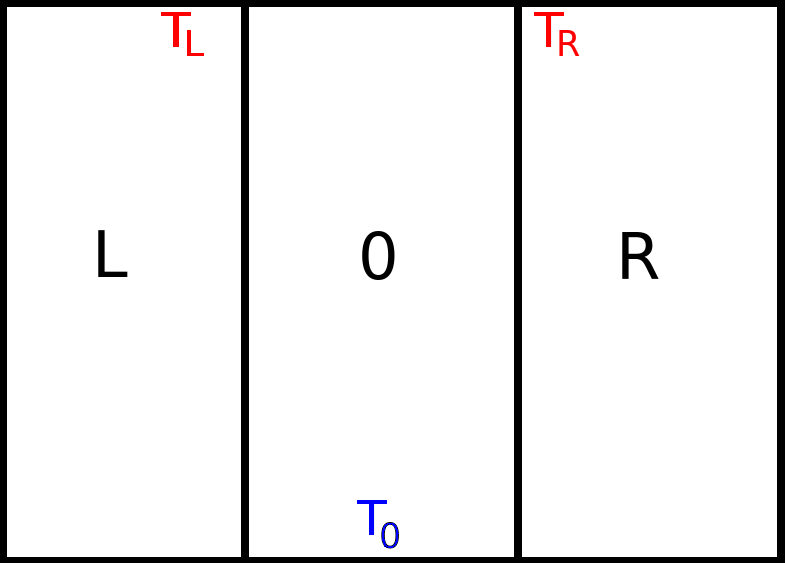
\includegraphics[width=0.4\linewidth]{multigrad}
\end{figure}
\pause\transsplitverticalout
\begin{exampleblock}{Redefine}
\[\Delta_t < \frac{c_v(T_u-T_0)}{R_L(\Delta_x,\Delta_t)+R_R(\Delta_x,\Delta_t) -
f_0c\sigma_p aT_0^4}\]
\[T_u = \mbox{max}(T_L,T_R)\]
\end{exampleblock}
\end{frame}

\subsection{Multigroup}
\begin{frame}\frametitle{Multigroup Approximation}
\begin{exampleblock}{}
\begin{align*}
\zeta &\equiv\int_0^\infty\frac{\sigma_0 B_u}{\hat\Sigma}
  \left(\frac{1}{2}-E_3(\hat\Sigma\Delta_x)\right) \\
&\approx\sum_{g=0}^G \frac{\sigma_{0,g} B_{u,g}}{\hat\Sigma_g}
  \left(\frac{1}{2}-E_{3,g}(\hat\Sigma_g\Delta_x)\right)
\end{align*}
\begin{align*}
f_g&\equiv\int_{\nu_g}^{\nu_{g-1}} f(\nu)\ d\nu 
\approx\sum_{n=1}^N \frac{f(\nu_n)+f(\nu_{n+1})}{2}
  \left(\nu_{n+1}-\nu_n\right),\\
&\hspace{200pt}\nu_g\leq\nu_n\leq\nu_{g-1}
\end{align*}
\end{exampleblock}
\end{frame}

\begin{frame}\frametitle{Multigroup Approximation}
\begin{columns}
\begin{column}{.5\textwidth}
\begin{figure}
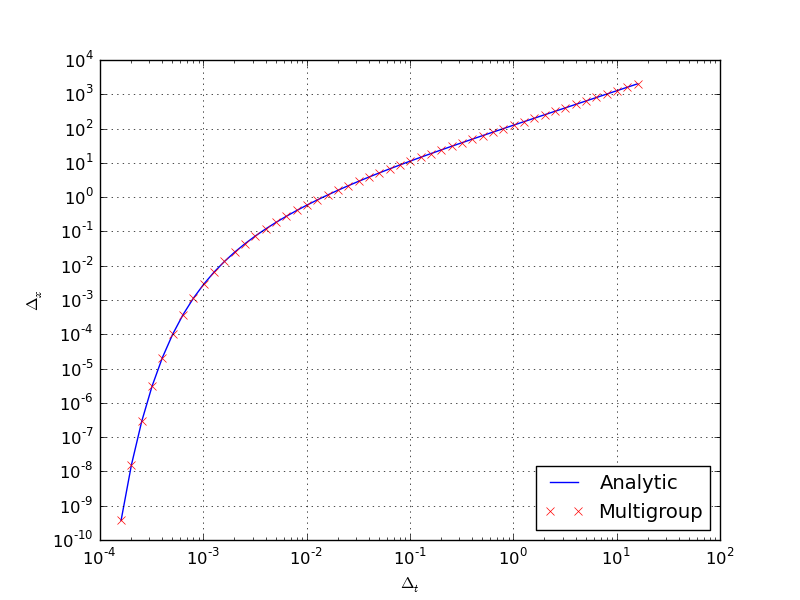
\includegraphics[width=\linewidth]{DMP_mg_numR}
\caption{Discrete Maximum Principle}
\end{figure}
\end{column}
\begin{column}{.5\textwidth}
\begin{figure}
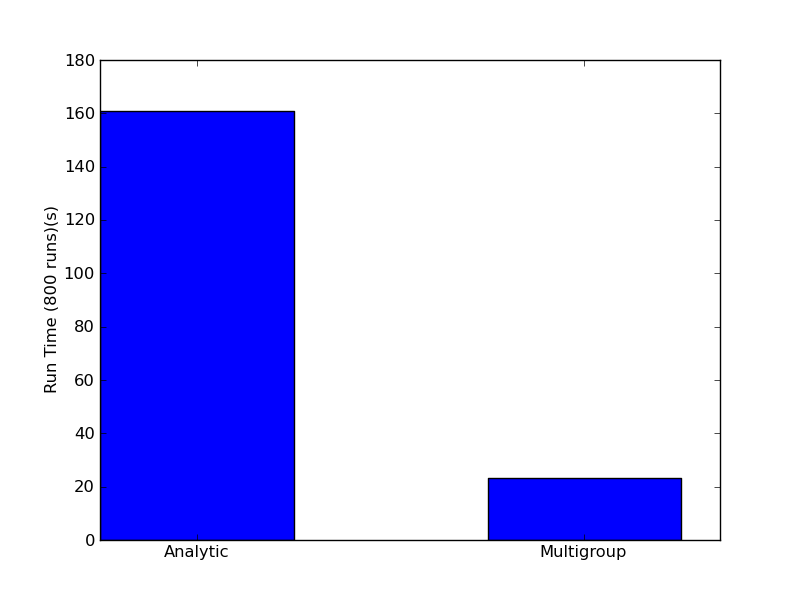
\includegraphics[width=\linewidth]{anl_mg_runtime}
\caption{Run Time Comparison}
\end{figure}
\end{column}
\end{columns}
\end{frame}



\section{Implementing the DMP}
\subsection{\texttt{draco}}
\begin{frame}\frametitle{Addition to \texttt{draco}}\label{origEiEn}
New functions: added \texttt{ExpInt.cc in}
\texttt{draco/special\_functions}:
\begin{block}{Ei$(x)$ \hyperlink{Ei_exp}{\beamergotobutton{more about this}}}
\begin{itemize}
 \item Approximates $\int\frac{e^{xt}}{t}dt$ to within machine
precision
  \item Uses extension Ei$(-x) = -E_1(|x|)$ for $x<0$
\end{itemize}
\end{block}

\begin{block}{$E_n(x)$ \hyperlink{En_exp}{\beamergotobutton{more about this}}}
\begin{itemize}
\item Approximates $\int\mu^{-n}e^{-x/\mu}\ d\mu$ to within $10^{-14}$.
\end{itemize}
\end{block}
\end{frame}


\subsection{\texttt{clubimc}}
\begin{frame}\frametitle{The DMP in \texttt{clubimc}}
\begin{block}{class: \texttt{DiscreteMaxPrinciple}}
\begin{itemize}
 \item Accepts cell-based material data
 \item Calculates DMP inequality
 \item Stores inequality value and pass/fail data
\end{itemize}
\end{block}
\begin{block}{class: \texttt{DMP\_Helper}}
\begin{itemize}
 \item Collects cell-based data from mesh, material state
 \item Generates vector of \texttt{DiscreteMaxPrinciple} objects
 \item Accesses limiting inequality value, cell index
\end{itemize}
\end{block}
\end{frame}

\begin{frame}\frametitle{The DMP in \texttt{clubimc}}
A Correction Occurs
\begin{columns}
\begin{column}{.5\textwidth}
\begin{figure}
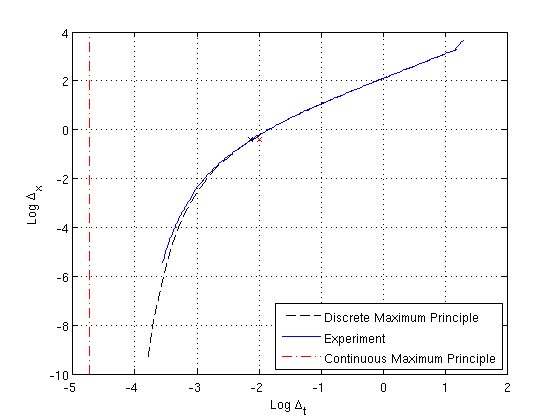
\includegraphics[width=\linewidth]{CMP_DMP}
\caption{Analytic DMP}
\end{figure}
\end{column}
\begin{column}{.5\textwidth}
\begin{figure}
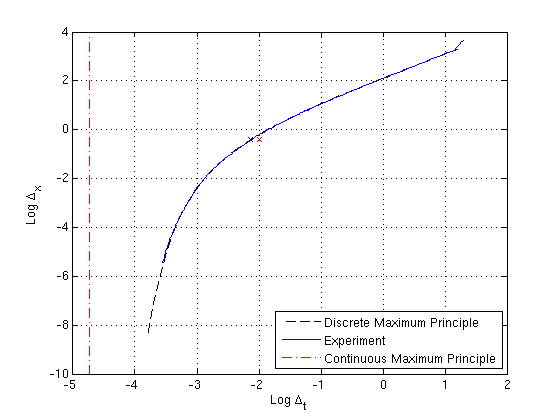
\includegraphics[width=\linewidth]{grossMG}
\caption{Multigroup DMP}
\end{figure}
\end{column}
\end{columns}
\end{frame}

\begin{frame}\frametitle{The DMP in \texttt{clubimc}}
\begin{tabular}{c c c c}
$\Delta_t$ & $\Delta_x$ & Expected & Calculated \\ \hline
$5.0596\times10^{-4}$ & $2.1\times10^{-4}$ & $3.74028\times10^{-6}$ &
  $3.74472\times10^{-6}$ \\
$1.6\times10^{-3}$ & $1.8\times10^{-2}$ & $3.23378\times10^{-5}$ &
  $3.23377\times10^{-5}$ \\
$1.6\times10^{-2}$ & $1.3\times10^{0}$ & $8.01371\times10^{-4}$ &
  $8.01372\times10^{-4}$ \\
$1.6\times10^{-1}$ & $1.95\times10^{1}$ & $5.69082\times10^{-3}$ &
  $5.69082\times10^{-3}$ \\
$1.6\times10^{0}$ & $2.1\times10^{2}$ & $8.31396\times10^{-2}$ &
  $8.31397\times10^{-2}$ \\
$1.6\times10^{1}$ & $2.1\times10^{3}$ & $7.33246\times10^{-1}$ &
  $7.33246\times10^{-1}$ \\ \hline
%%%%%%%%%%%%%%%%%%%%%%%%%%%%should violate v, should not ^
$5.0596\times10^{-4}$ & $1.9\times10^{-4}$ & $-5.36018\times10^{-6}$ &
  $-5.35573\times10^{-6}$ \\
$1.6\times10^{-3}$ & $1.6\times10^{-2}$ & $-3.94675\times10^{-5}$ &
  $-3.94676\times10^{-5}$ \\
$1.6\times10^{-2}$ & $1.1\times10^{0}$ & $-1.29592\times10^{-3}$ &
  $-1.29592\times10^{-3}$ \\
$1.6\times10^{-1}$ & $1.8\times10^{1}$ & $-6.81044\times10^{-3}$ &
  $-6.81043\times10^{-3}$ \\
$1.6\times10^{0}$ & $1.9\times10^{2}$ & $-7.71581\times10^{-2}$ &
  $-7.71580\times10^{-2}$ \\
$1.6\times10^{1}$ & $1.9\times10^{3}$ & $-8.60397\times10^{-1}$ &
  $-8.60396\times10^{-1}$ 
\end{tabular}
\end{frame}


\begin{frame}\frametitle{.}
{}
\end{frame}


%extra info pages, don't want included in the main
\appendix
\section{Appendix: More about Exponential Function Implementation}
\begin{frame}\frametitle{More about Ei$(x)$ Implementation}
\label{Ei_exp}
\begin{exampleblock}{$x\leq\log{\epsilon}\sim36$ Power Series}
\[\mbox{Ei}(x)=\gamma + \ln{x} + x + \frac{x^2}{2\cdot2!}+...\]
\end{exampleblock}
\begin{exampleblock}{$x>\log{\epsilon}$ Asymptotic Expansion}
\[\mbox{Ei}(x)\sim\frac{e^x}{x}\left(1+\frac{1}{x}+\frac{2!}{x^2}+...\right)\]
\end{exampleblock}
\hyperlink{origEiEn}{\beamerreturnbutton{return}}
\end{frame}

\begin{frame}\frametitle{More about $E_n(x)$ Implementation}
\label{En_exp}
\begin{exampleblock}{$x<1$ Digamma Series}
\[E_n(x)=\frac{(-x)^{n-1}}{(n-1)!}[-\ln(x)+\psi(n)] -
  \sum_{m\neq n-1}^\infty\frac{(-x)^m}{(m-n+1)m!}\]
\[\psi(n)\equiv-\gamma+\sum_{m=1}^{n-1}\frac{1}{m}\]
\end{exampleblock}
\begin{exampleblock}{$x\geq1$ Continued Fraction}
\[
E_n(x)=\cfrac{e^{-x}}{x+n
                     - \cfrac{n}{x+n+2
                     - \cfrac{2(n+1)}{x+n+4-...}}}
\]
\end{exampleblock}
\hyperlink{origEiEn}{\beamerreturnbutton{return}}
\end{frame}


\end{document}




